% !TeX root = ../main.tex

\section{Results}
    \frame{\sectionpage}

    \begin{frame}{Running time of Benders Decomposition and IP}
        \scriptsize
        \begin{table}[ht]
            \centering
            \begin{tabular}{|l|l|l|l|l|l|l|}
            \hline
            \# of scenarios & demands & running time of IP(s) & Benders (s) & \# of rows & \# of groups & \# of seats\\
            \hline
            1000  & (150, 350) & 5.1  & 0.13 & 30 & 8 & (21, 50)\\
            5000  & & 28.73 & 0.47 & 30 & 8 \\
            10000 & & 66.81  & 0.91 & 30 & 8 \\
            50000 & & 925.17 & 4.3 & 30 & 8 \\
            \hline
            1000  & (1000, 2000) & 5.88 & 0.29 & 200 & 8 & (21, 50)\\
            5000  & & 30.0 & 0.62 & 200 & 8 \\
            10000 & & 64.41 & 1.09 & 200 & 8 \\
            50000 & & 365.57 & 4.56 & 200 & 8 \\
            \hline
            1000  & (150, 250) & 17.15  & 0.18 & 30 & 16 & (41, 60) \\
            5000  & & 105.2  & 0.67 & 30 & 16  \\
            10000 & & 260.88 & 1.28 & 30 & 16  \\
            50000 & & 3873.16 & 6.18 & 30 & 16  \\
            \hline
            \end{tabular}
          \end{table}
    \end{frame}
      
    \begin{frame}{Feasible Seat Planning versus IP Solution}
        \scriptsize
        \begin{table}[ht]
            \begin{tabular}{|l|l|l|l|l|l|}
            \hline
            \# samples & T & probabilities & \# rows & people served by FSP & IP \\
            \hline
            1000  & 45  & [0.4,0.4,0.1,0.1] & 8 & 85.30 & 85.3 \\
            1000  & 50  & [0.4,0.4,0.1,0.1] & 8 & 97.32 & 97.32 \\
            1000  & 55  & [0.4,0.4,0.1,0.1] & 8 & 102.40 & 102.40  \\ % slow
            1000  & 60  & [0.4,0.4,0.1,0.1] & 8 & 106.70 & NA  \\
            1000  & 65  & [0.4,0.4,0.1,0.1] & 8 & 108.84 & 108.84 \\
            \hline
            1000  & 35  & [0.25,0.25,0.25,0.25] & 8 & 87.16 & 87.08 \\
            1000  & 40  & [0.25,0.25,0.25,0.25] & 8 & 101.32 & 101.24 \\
            1000  & 45  & [0.25,0.25,0.25,0.25] & 8 & 110.62 & 110.52 \\
            1000  & 50  & [0.25,0.25,0.25,0.25] & 8 & 115.46 & NA \\
            1000  & 55  & [0.25,0.25,0.25,0.25] & 8 & 117.06 & 117.26 \\
            \hline
            5000  & 300  & [0.25,0.25,0.25,0.25] & 30 & 749.76 & 749.76 \\
            5000  & 350  & [0.25,0.25,0.25,0.25] & 30 & 866.02 & 866.42 \\
            5000  & 400  & [0.25,0.25,0.25,0.25] & 30 & 889.02 & 889.44 \\
            5000  & 450  & [0.25,0.25,0.25,0.25] & 30 & 916.16 & 916.66 \\
            \hline
            \end{tabular}
        \end{table}

    Each entry of people served is the average of 50 instances.
    IP will spend more than 2 hours in some instances, as `NA' showed in the table.
    \end{frame}
      
    \begin{frame}{Results of Different Policies}
        \scriptsize
        \begin{table}[ht]
          \centering
          \caption{Results of different policies}
          \begin{tabular}{|l|l|l|l|l|l|}
          \hline
           T & probabilities & Sto(\%) & DP1(\%) & Bid-price(\%) & FCFS(\%) \\
          \hline
           60  & [0.25, 0.25, 0.25, 0.25]  & 99.12 & 98.42 & 98.38 & 98.17 \\
           70  & [0.25, 0.25, 0.25, 0.25]  & 98.34 & 96.87 & 96.24 & 94.75 \\
           80  & [0.25, 0.25, 0.25, 0.25]  & 98.61 & 95.69 & 96.02 & 93.18 \\
           \hline
           60  & [0.25, 0.35, 0.05, 0.35]  & 98.94 & 98.26 & 98.25 & 98.62 \\
           70  & [0.25, 0.35, 0.05, 0.35]  & 98.05 & 96.62 & 96.06 & 93.96 \\
           80  & [0.25, 0.35, 0.05, 0.35]  & 98.37 & 96.01 & 95.89 & 92.88 \\
          \hline
          60  & [0.15, 0.25, 0.55, 0.05]  & 99.14 & 98.72 & 98.74 & 98.07 \\
          70  & [0.15, 0.25, 0.55, 0.05]  & 99.30 & 96.38 & 96.90 & 96.25 \\
          80  & [0.15, 0.25, 0.55, 0.05]  & 99.59 & 97.75 & 97.87 & 95.81 \\
          \hline
          \end{tabular}
        \end{table}

          We compare the performance of different policies to the optimal value. Specifically, we consider two policies for seat assignment after all group arrivals: DSA and FCFS. In addition, we evaluate two policies for seat assignment for each group arrival: one based on dynamic programming (DP) and the other based on first-come, first-served (FCFS) scheduling.
    \end{frame}
      
    \begin{frame}{Result of Different Demands}
        \small
        Let $c = p_1 * 1 + p_2 * 2 + p_3 * 3 + p_4 * 4$ denote the number of people each period.
        \begin{figure}[h]
            \centering
            \subfigure[When $\gamma =2.5$]{
              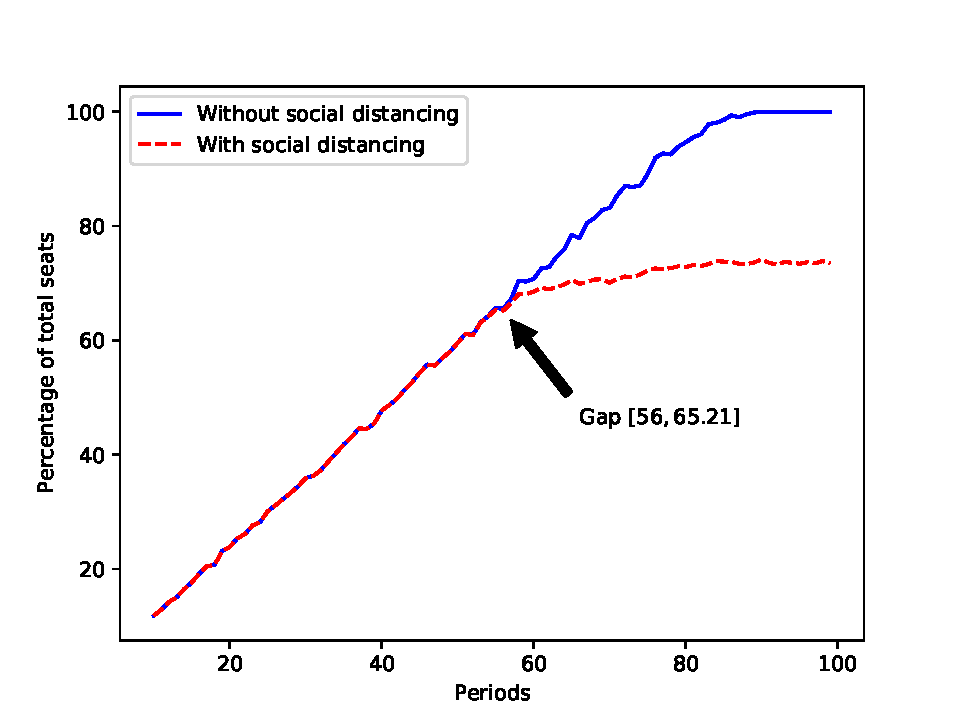
\includegraphics[width=0.48\textwidth]{./images/p1.pdf}}
            \subfigure[When $\gamma =1.9$]{
              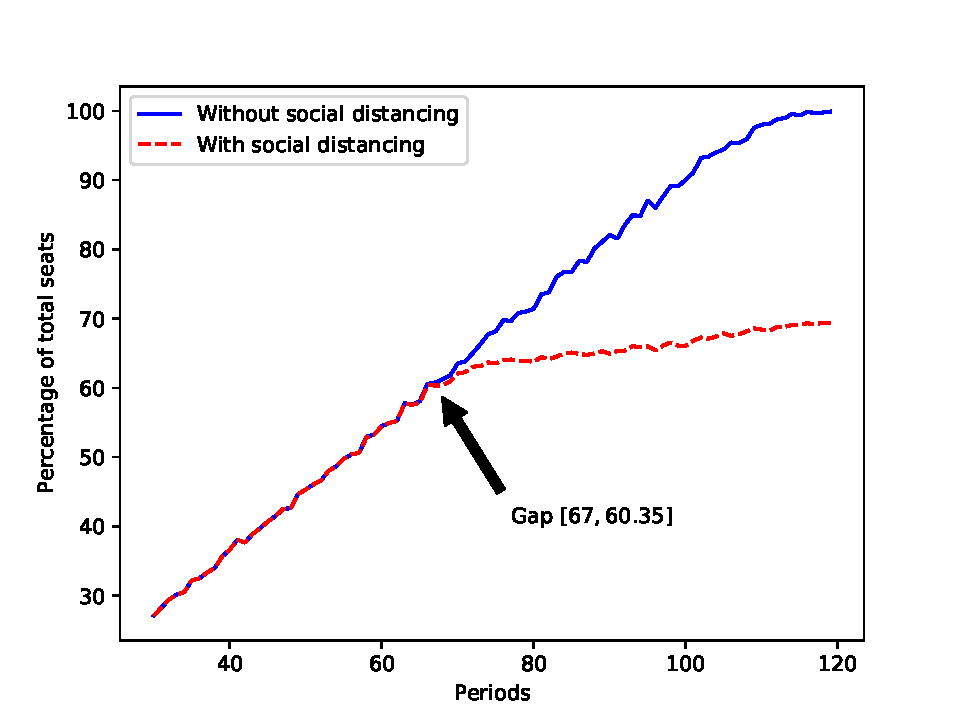
\includegraphics[width=0.48\textwidth]{./images/p2.pdf}}
          \end{figure}

        The gap point represents the first period where the number of people without social distancing is larger than that with social distancing and the gap percentage is the corresponding percentage of total seats.
    \end{frame}
      
    \begin{frame}{Results of the Number of Arriving People per Period}
        
        \begin{figure}[ht]
            \centering
            \subfigure[One instance for each probability combination]{
              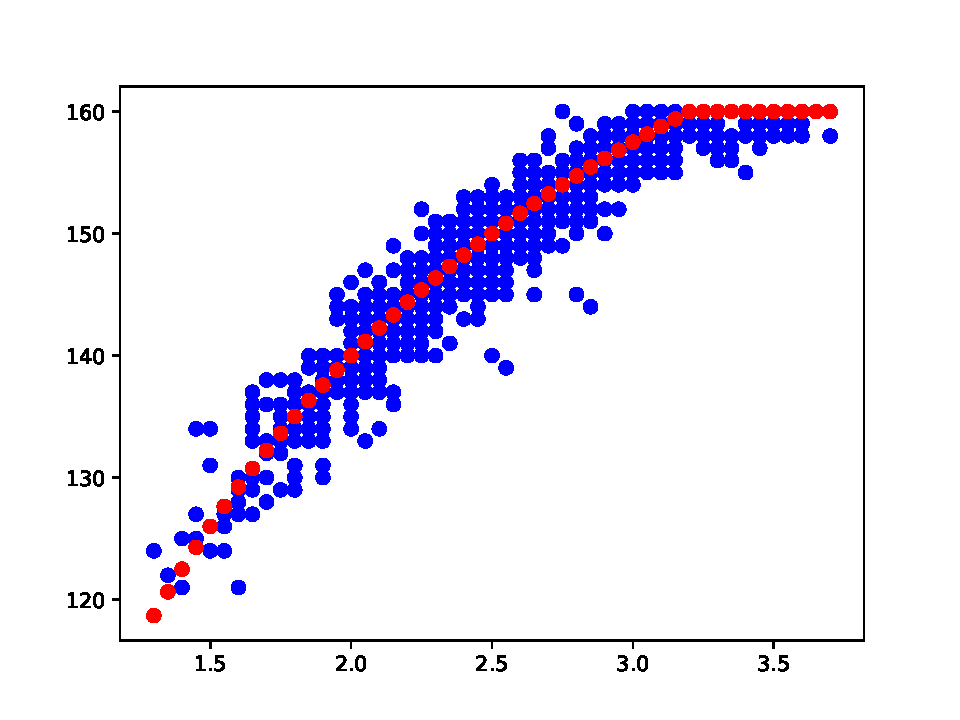
\includegraphics[width=0.48\textwidth]{./images/diff_1.pdf}}
            \subfigure[Average of 50 instances for each probability combination]{
              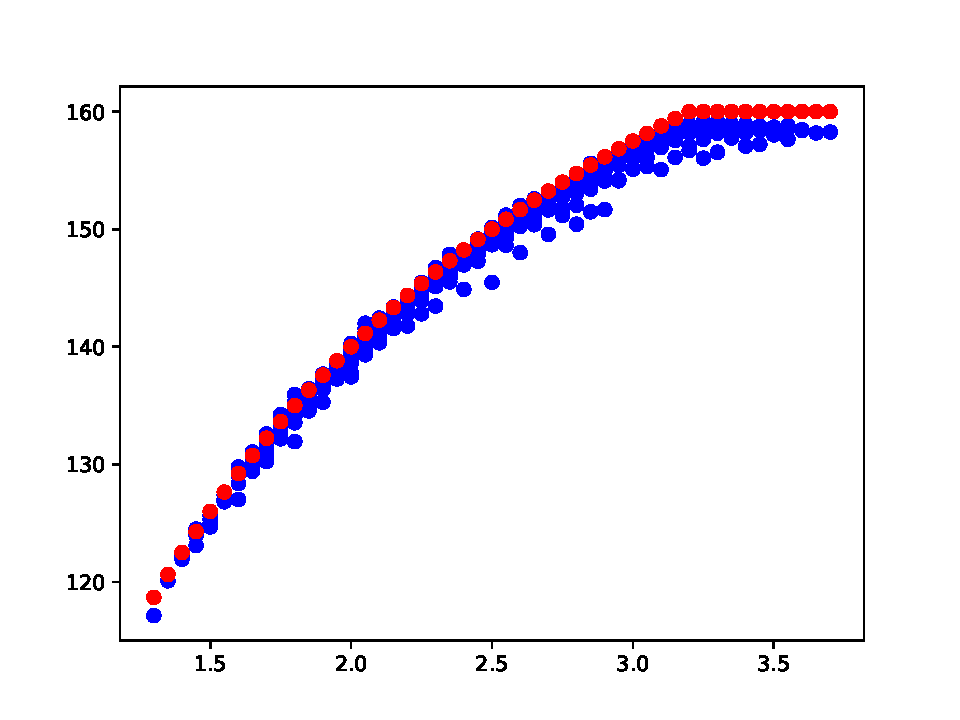
\includegraphics[width=0.48\textwidth]{./images/diff_2.pdf}}
            \caption{The number of people served versus $c$}
          \end{figure}

    \end{frame}
      
      
    \begin{frame}{Results of Different Seat Layouts}
        \begin{figure}[ht]
            \centering
            \subfigure[Average of 50 instances for step-size seat layout]{
              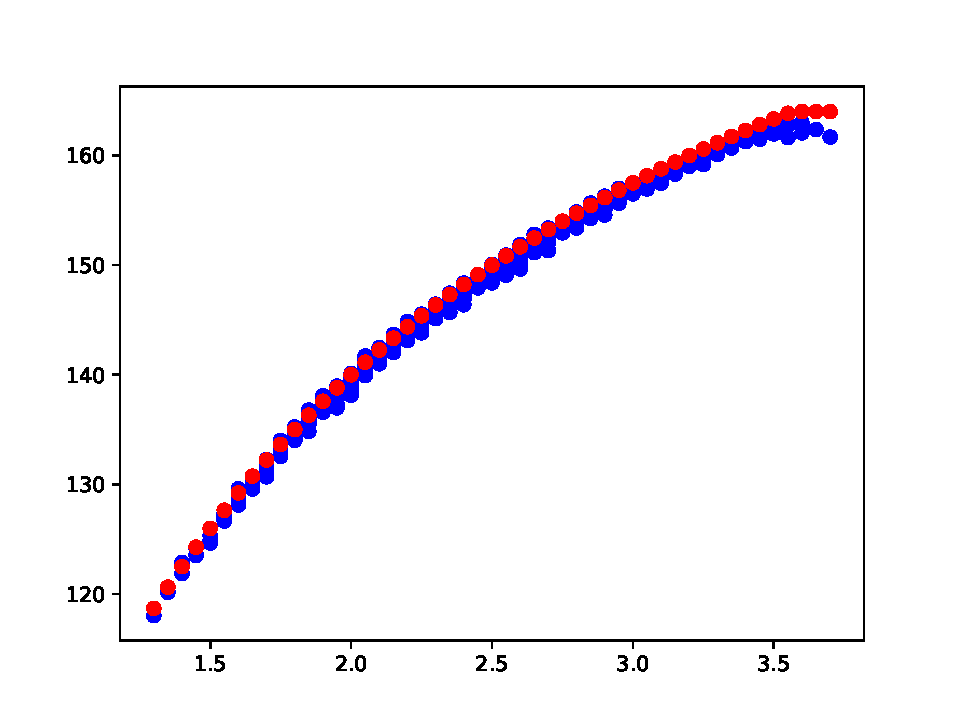
\includegraphics[width=0.48\textwidth]{./images/stepsize_seat.pdf}}
            \subfigure[Average of 50 instances for random seat layout]{
              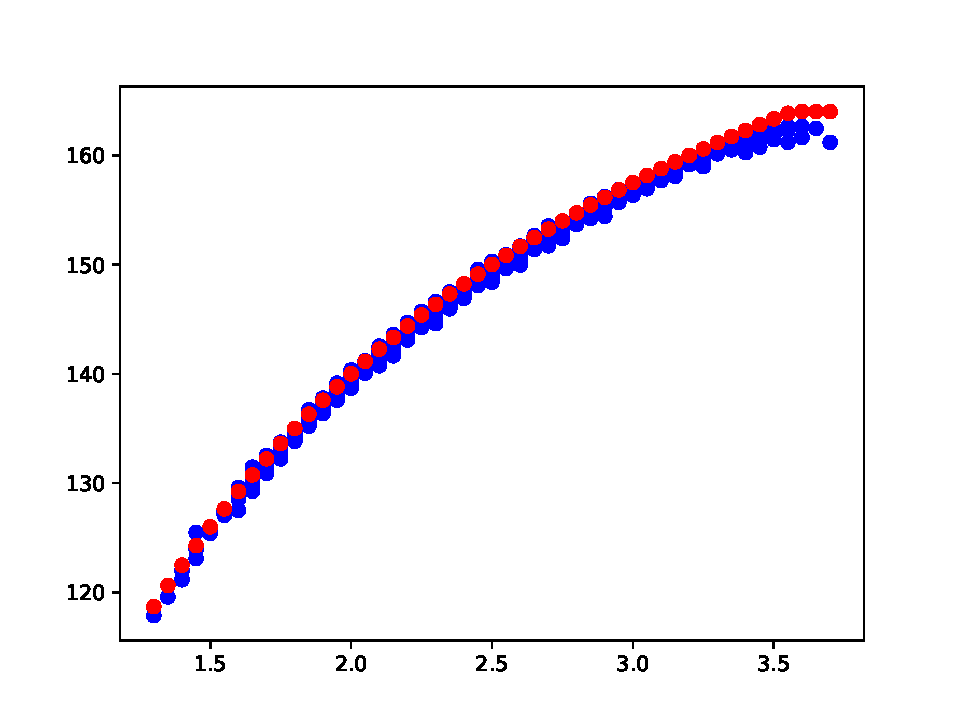
\includegraphics[width=0.48\textwidth]{./images/random_seat.pdf}}
            \caption{The number of people served versus $c$}
          \end{figure}

    \end{frame}
      


